\documentclass[10pt a4paper twoside]{report}

\usepackage{ragged2e}
\usepackage{tikz, pgfplots}
\usepackage{graphicx}
\usepackage{multicol}
\usetikzlibrary{positioning,shapes}
\usepackage{graphicx}
\graphicspath{{./reportImages/}}
\usepackage{geometry}
\usepackage{listings}
\usepackage{amsmath}
%\usepackage[usenames,dvipsnames]{xcolor} % to access some named colors used with \highLight
%\usepackage{luacolor} % required to use the lua-ul \highLight command
%\usepackage{lua-ul}

%\LuaULSetHighLightColor{Aquamarine}

\geometry{margin=1in}

\lstdefinestyle{st1}{
	numbers=left,
	tabsize=2
}

\lstset{style=st1}

\title{Optimizing Computational Graphs Using Relaxed Graph Substitutions}

\author{Kaushik Bhowmick\\ \texttt{u21cs022@coed.svnit.ac.in}
		\and
		Himanshu Thakur\\ \texttt{u21cs046@coed.svnit.ac.in}
		\and
		Bhavya Hirani\\ \texttt{u21cs100@coed.svnit.ac.in}
		}

\date{\today}

\begin{document}
\maketitle

%\begin{center}
%{ \Large \bfseries Building a test case for Interprocedural GVN } \\
%\end{center}

\begin{abstract}

	Most deep learning compilers use a greedy approach to optimizing computational graphs in that every successive graph substituion must result in a strict performance increase. This narrows the space of possible optimizations and motivates the notion of relaxed graph substitutions: substitutions that don't themselves result in a more optimal graph version, but facilitate further transformations down the line that ultimately yield a net improvement in performance. In order to determine the pipeline of transformations to be applied such that the net performance increase is guaranteed, we search the space of potential optimizations using a backtracking algorithm which, at a given iteration, determines the cost of the corresponding intermediate graph using programmer-defined heuristics. To test our optimization strategy, we plan to use the set of graph transformations available in TensorFlow's repository and we limited our performance heuristics to simply measuring execution time. Our work is based on the strategy presented in \cite{jia2019}.\\

\end{abstract}

\chapter{Introduction}
%{\large \noindent \bfseries  Introduction}\\

We use an example from a ResNet \cite{he2016} module ( figure \ref{resnet} ) to illustrate our strategy. Each arrow represents a graph substitution that produces a graph \textit{equivalent} to its input, where equivalence is defined as the following: two graphs $\mathcal{G}_1$ and $\mathcal{G}_2$ are said to be equivalent if they produce the same outputs for an arbitary input. The first substitution pads a 1x1 convolutional kernel to form a 3x3 one, potentially reducing the performance by introducing more operations. However, doing so enables further node fusions which, as we can see, results in a computational graph giving better performance than what we started with. \\


\begin{figure}[b!]
	\begin{center}
		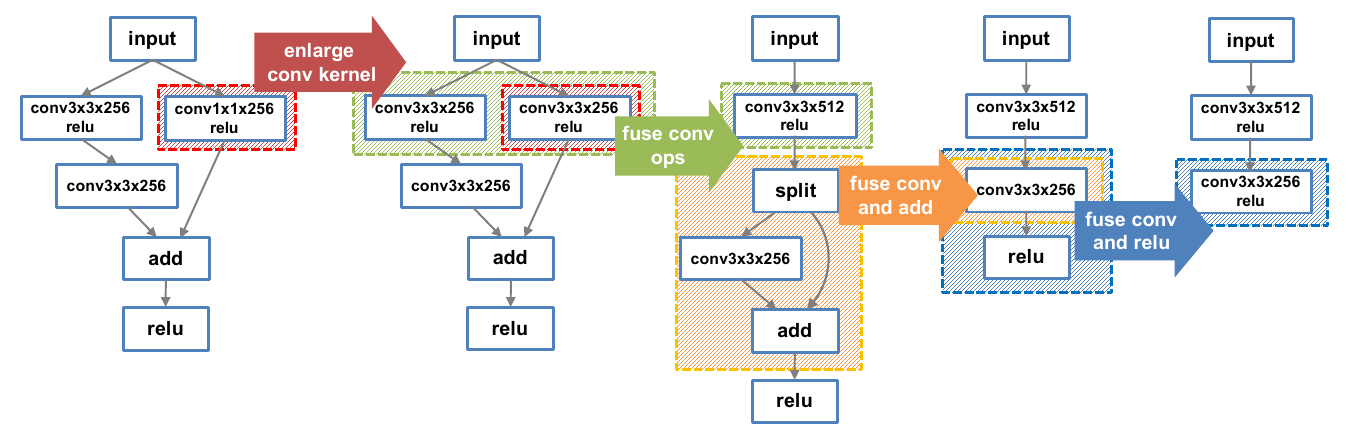
\includegraphics[scale=0.3]{resnetExample}
	\end{center}	
	\caption{An example from \cite{jia2019} that demonstrates a relaxed graph substitution}
	\label{resnet}
\end{figure}

%\pagebreak

\chapter{Theoretical Background and Literature Review}
%{\large \noindent \bfseries  The Backtracking Algorithm}\\



%{\large \noindent \bfseries  Proposed Methodology}\\
\chapter{Proposed Algorithm and Future Directions}

	\section{Motivating our Approach Using an Example}
		% overview of the resnet example
		% emphasize that after every transform, semantics shouldn't be sacrificed

	\section{The backtracking Algorithm}

		We take the following approach to search through the space of possible graph transformations:
		\begin{enumerate}
			\item Consider a list of possible graph transformations, $T$. At any given point in the algorithm, let $\mathcal{G}$ be the current intermediate graph version. We maintain a priority queue of intermediate graphs, ordered by their \textit{cost}, defined by a heuristic (in our case, this is simply the execution time).
			\item In each iteration:
				\begin{enumerate}
					\item We dequeue to get the next candidate intermediate representation $\mathcal{G}$. 
					\item For each optimization $t_i$ in $T$, we apply $t_i$ on $\mathcal{G}$ to obtain some equivalent graph $\mathcal{G}'$. If $cost(\mathcal{G}') < cost(\mathcal{G})$, we set $\mathcal{G} = \mathcal{G}'$. Else if $cost(\mathcal{G}') < \alpha \cdot cost(\mathcal{G})$, where $\alpha$ is a hyperparameter defined by the user (greater than one), then $\mathcal{G}'$ is considered to be a valid candidate for further search, and is added to the priority queue.
					\item $\alpha$ helps define how much of a performance decrease we can tolerate. This value can't be too high so as to avoid blowing up the search space, and hence, the time it takes for our algorithm to find a beneficial sequence of graph transformations.
				\end{enumerate}

			\item The above is repeated until there are still graphs to process in the queue.

		\end{enumerate}
	\section{Diving Into the Transformations}
		% tensorflow didn't have transforms we could work off of, so went with the paper's example
		% deep dive in the transforms
		\subsection{Kernel Expansion and Fusing Convolutions}
		\subsection{Fusing Split and Add Nodes}

	\section{The Cost Model}
		
		% Explain the need for evaluating it statically
		% FLOPS
		% Execution time

	\section{Implementation Strategy and Future Work}

		\subsection{Regarding the Backtracking Algorithm}

		\subsection{Implementing Transformations for ONNX}

		\subsection{Fleshing Out the Cost Model}

\chapter{Conclusion}

%\begin{enumerate}

	%\item The first step would be to finalize a set of graph transformations we will be working with (i.e. the set $T$ in the earlier algorithm). We initially construted the initial computation graph shown in figure \ref{resnet} using the ONNX Python API \cite{onnxpython}, and explored the graph transformations made available by the ONNX Optimizer \cite{onnxoptimizer} through a simple backtracking algorithm. That being said, since ONNX provides \textit{optimizations} and not \textit{transformations}, each available transform is bound to improve performance for most if not all input graphs. This renders the purpose of our algorithm moot. This is why, we now plan to explore the transformations made available through the TensorFlow \cite{tf2016} API which also provides a tool to write custom transforms.
	%\item Once a set of Tensorflow transforms are shortlisted, we can move on to analyze the feasibility of, and then potentially implement, the two latter transforms mentioned in figure \ref{resnet}, which currently don't have implementations in TensorFlow. 
	%\item We then create a test suite consisting of small computation graphs that demonstrate the abilities of our algorithm.
	%\item Once the aforementioned stages are successful, we will then benchmark our backtracking implementation against the aforementioned test suite, and analyze the results.
	%\item Based on the results obtained, we then aim to tweak the cost model that approximates the cost function for an input graph so as to consider other parameters such as FLOPS or memory consumed.
	%\item The above steps will hopefully yield a model that is successful with regard to small input computation graphs. In order to scale this system to work for existing models, which have massive computation graphs that are bound to blow up the search space exponentially, we plan to create a \textit{graph splitting} algorithm that divides the computation graph into smaller sub-graphs. Each sub-graph can then be optimized through the earlier algorithm. In \cite{jia2019}, the metric used to find partitioning-boundaries is a parameter called $Cap(N)$, which, for a given node $N$, tells us the number of graph transformations thwarted if the graph were split through this node. Since we want the least number of thwarted transforms, the paper then uses the max-flow algorithm \cite{cormen2009introduction} to find partitioning boundaries.
	%\item The paper also mentioned that this min-cut algorithm is not necessarily optimal for all models. Hence, there is scope of improvement with regard to defining better graph-splitting heuristics. We see this as possible future work.

%\end{enumerate}


\bibliographystyle{plain}
\bibliography{refs}

\begin{center}
\begin{tabular}{@{}p{.5in}p{4in}@{}}
& \hfill \\
& \hfill \\
& \hrulefill \\
& Shri. R. P. Gohil \\
& Associate Professor, DoCSE, SVNIT\\
\end{tabular}
\end{center}

\end{document}
